% 1章
\chapter{序論}
\label{chap:introduction}
%
%\input{introduction/preface}
%
%!TEX root = ../thesis.tex

\section{背景}
AIFormulaは計測自動制御学会と自動車技術会が主催し, 本田技術研究所がサポートする次世代の人工知能モビリティの競技会で, 正式な競技会は2025年から始まる.
\cite{aiformula}
AIFormulaは今後ますます需要が高まるであろう自動化システムの技術者を育てるという点で効果が見込まれる.
AIFormulaではハードウェアの変更もある程度許容されているが, 現時点での開発はソフトウェアが中心となる.
ハードウェアは経路追従するために必要なパーツが全て揃っているが, ソフトウェアはデバイスを駆動するサンプルプログラムが用意されているのみである.
\cite{aiformula-support}
競技という性質上, 経路追従などのソフトウェアは各チームで開発することが必要となる.
\cite{aiformula-chibakou}
\cite{aiformula-repo}
その点で, コースを自動で走行するためにはソフトウェアの開発は必須となる.

\subsection{ハードウェア}
AIFormulaでは詳細なルールは検討中であるとのことで, 2025年2月に開催される予定のプレ大会以降に詳細なルールが決定される予定となっている.
Fig.1.1に2025年のプレ大会で使用される予定のロボットを示す.
ロボットは本田技術研究所から貸与されたロボットを使用していて, 差動二輪と一輪のキャスタ(以下, 従動輪と呼ぶ)で構成された三輪モデルである.
バッテリーにはMPP(Mobile Power Pack)が使用される. MPPは持ち運び可能な交換式バッテリーとなっている. Fig.1.2にMPPを示す.
プレ大会では指定されたコースを3周する時間で競われる.

\begin{figure}[H]
  \centering
 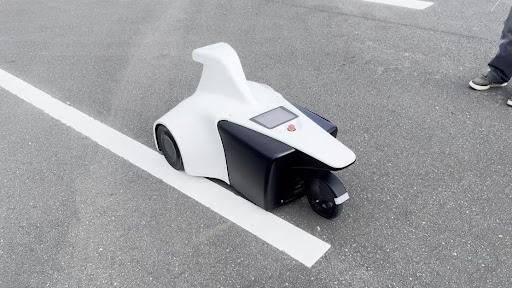
\includegraphics[keepaspectratio, scale=0.6]
      {images/ExteriorViewOfTheMobilityPlatform.png}
 \caption{Exterior view of the mobility platform}
 \label{fig:robot view}
\end{figure}

\begin{figure}[H]
  \centering
 \includegraphics[keepaspectratio, scale=0.08]
      {images/mpp.png}
 \caption{Mobile Power Pack}
 \label{fig:MPP}
\end{figure}

\subsection{レギュレーション}
詳細なルールは検討中の段階であるが, Table.1.1に現時点で判明しているレギュレーションについて示す.

\begin{table}[H]
     \centering
     \caption{regulation}
     \begin{tabular}{|c|c|lll}
     \cline{1-2}
                              & レギュレーション              &  &  &  \\ \cline{1-2}
                                   & 車体寸法, モータ, バッテリー(MPP), タイヤは統一 &  &  &  \\
     ハードウェア                       & 三輪モデル(差動二輪+従動輪)               &  &  &  \\
                                   & LiDAR使用禁止                     &  &  &  \\
                                   & 一部基板ソフトウェア変更不可                &  &  &  \\ \cline{1-2}
     \multicolumn{1}{|l|}{ソフトウェア} & 高精度地図の使用禁止                    &  &  &  \\
     \multicolumn{1}{|l|}{}       & Autowareパッケージの使用禁止            &  &  &  \\ \cline{1-2}
     \end{tabular}
\end{table}

\subsection{コース}
Fig.1.3にAIFormulaのコースを示す.
周囲に高い建造物のない平坦なコースである.


\begin{figure}[H]
  \centering
 \includegraphics[keepaspectratio, scale=0.1]
      {images/AerialViewAndMobilitysPerspetiveOfTheCourse.png}
 \caption{Aerial view and mobility perspective of the course}
 \label{fig:course}
\end{figure}


\section{目的}
本研究では, 経路追従をするパッケージを開発して評価を行うことで作成した経路追従ソフトウェアの有効性を実環境で検証することを目的とする.


\section{論文の構成}
本論文は以下のように構成される.
まず, 2章で本研究で使用される要素技術について述べる.
3章では経路追従する際に使用するアルゴリズムについて述べる.
4章では開発した経路追従ソフトウェアに要求されるシステムについてまとめる.
5章ではシミュレータ環境で経路追従の実験を行い, アルゴリズムの有効性を確認する.
6章では実環境で経路追従の実験を行う.
7章では本研究の結論をまとめる.

\newpage

% 2章
\chapter{要素技術}
本章では, 本研究に関連する要素技術を述べる.
%!TEX root = ../thesis.tex

\section{ROS 2}
ROS 2(Robot Operating System versition 2)\cite{ros2}は, オープンソースのロボットソフトウェアフレームワークであり,
ロボットアプリケーションの開発や実行をサポートするミドルウェアである.
異なるバージョンが存在しているが, 本研究ではROS 2 foxyを主に使用している.

\subsection{RViz2}
RViz2(ROS VIsualization 2)\cite{rviz}はROS 2で提供される三次元ビジュアライゼーションツールであり, 
数値で表されるロボットの座標や各センサのデータを視覚的に表すことができる.

\begin{figure}[H]
  \centering
 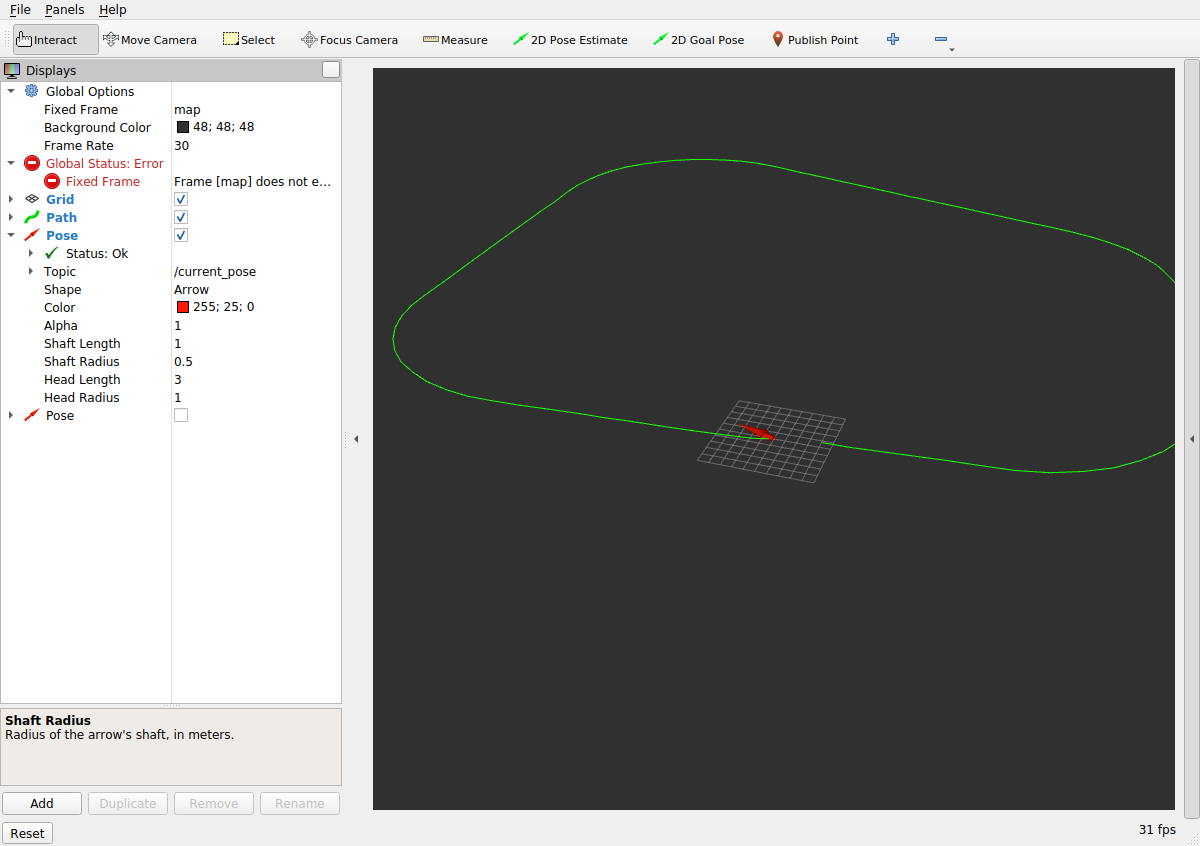
\includegraphics[keepaspectratio, scale=0.4]
     {images/rviz.png}
 \caption{RViz2 view}
 \label{fig:purepursuit}
\end{figure}

\section{GNSS}
GNSS(Global Navigation Satelite System)は, 
人工衛星を利用して地上の現在位置を計測するためのシステムであり, 
アメリカのGPS, ロシアのGLONASS, ヨーロッパのGalileo, 日本のQGSSなどを総称した衛生測位システムを指す.

計測する値は衛生と受信機(アンテナ)間の距離であり, 衛生位置を既知として受信機の三次元座標と受信機時計の誤差を未知数として最低4つの観測値から座標計算される.
測定された距離にはさまざまな誤差要因が含まれる.

\subsection{UTM座標系}
UTM(Universal Transverse Mercator)座標系\cite{utm}とは, 全世界を経度6度ごとのゾーンに分けて東回りに番号を付けて規格化したものである.
世界的にも大・中縮尺の図法として採用され, 日本では国土地理院の地形図や地勢図で採用されている.

\begin{figure}[H]
  \centering
 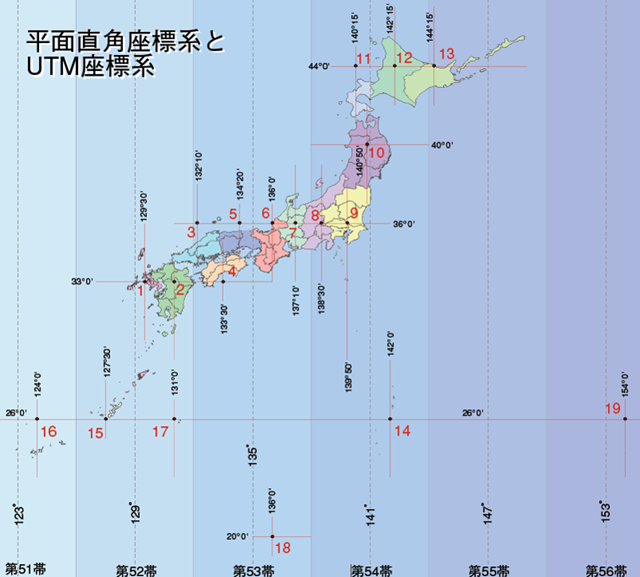
\includegraphics[keepaspectratio, scale=0.7]
      {images/UTMCoordinateSystem.png}
 \caption{UTM Coordinate System(source : [7]}
 \label{fig:UTM}
\end{figure}

% AIFormulaの会場となるAIモビリティパークは茨城県常総市にあるため, 54帯のUTM座標系を使用する.

\subsection{ECEF座標系}
ECEF(Earth-Centered, Earth-Fixed)座標系とは, 地理的・直交的な座標系であり, 地球の自転と同期して常時回転している座標系である.

\subsection{測地座標系}
測地座標系とは, 地球上の位置を緯度, 経度, および回転楕円体からの高さで表す座標系である.

\subsection{マルチパス}
マルチパスとは, 電波がまっすぐに届くだけでなくビルなどの高層建造物に反射して複数のルートを通って伝播することである.
反射した電波は到達するまでにわずかな遅れを生じ, 遅れの時間の分だけ距離が遠いと計測されてしまうため, 正確な測位を乱す要因の一つとなっている.

\begin{figure}[H]
  \centering
 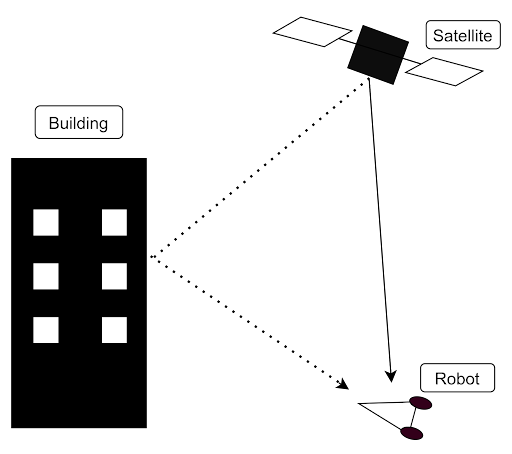
\includegraphics[keepaspectratio, scale=0.4]
      {images/multipath.png}
 \caption{Multipath}
 \label{fig:multipath}
\end{figure}

\section{IMU}
IMU(Inertial Measurement Unit)は, 
3次元の慣性運動を検出する装置である. 
加速度センサーにより並進運動を検出し, 
ジャイロセンサーにより回転運動を検出することができる.

\section{PID制御}
PID制御(Proportional-Integral-Differential Controller)は, 制御工学におけるフィードバック制御の一種である.
出力値と目標値との偏差, その積分, および微分の3つの要素によって, 入力値の制御を行う方法である.

\subsection{P制御}
基本的なフィードバック制御として比例制御(P制御)がある.
これは操作量を制御量と目標値の偏差の一次関数として制御するものである.
PID制御では, この偏差に比例して操作量を変化させる動作を比例動作, またはP動作といい, その時の定数は比例ゲイン, Pゲインと呼ばれる.

\subsection{I制御}
P制御において, 周囲の環境が変わるたびに残留偏差をなくすように比例ゲインを決定しなおすことが難しい.
そこで, 残留偏差が存在する場合, その偏差の時間積分に比例して入力値を変化させる動作をする項を追加する.
追加した項が持つ役割がI制御である.
偏差のある状態が長い時間続けばそれだけ入力値の変化を大きくして目標値に近づけようとする役目を果たす.
ここで, 定数は積分ゲイン, Iゲインと呼ばれる.

\subsection{D制御}
PI制御の問題点として, 周囲の環境が変化したり制御対象に撹乱が加わったりすることで出力値が急に変動することがある.
この問題を解決するために, 急激な出力値の変化が起こった場合, その変化の大きさに比例した入力を行うことでその変化に抵抗する役割を持つ項を追加する.
追加した項が持つ役割がD制御である.
定数は微分ゲイン, Dゲインと呼ばれる.

\newpage
% 3章
\chapter{経路追従に用いるアルゴリズム}
本章では, 経路追従に用いるアルゴリズムについて述べる.
%!TEX root = ../thesis.tex

\section{経路追従}
経路追従(Path following)とは, 経路計画(Path planning)で引いた経路に対して安全にロボットが経路を追従できるようにロボットを制御することである.
基本的にはロボットのモデルと制御アルゴリズムを利用することで, 最終的にロボットの入力値(ステアリング角度や並進速度)を計算することが目的となる.

\subsection{PurePursuit}
PurePursuitアルゴリズムは, 経路追従アルゴリズムの中で最も基礎的だが, 非常に広く使われているアルゴリズムである.

PurePursuitはFig.3.1に示すように目標経路上(Path)に対して一定距離先の点を目標点(Look Ahead)とし, その点に到達するようなステアリング制御を行う.
目標点に対してロボットが前進することで, より先の目標点にたどり着くように制御を行うため, 結果的に目標経路に追従する形となる.

\begin{figure}[H]
  \centering
 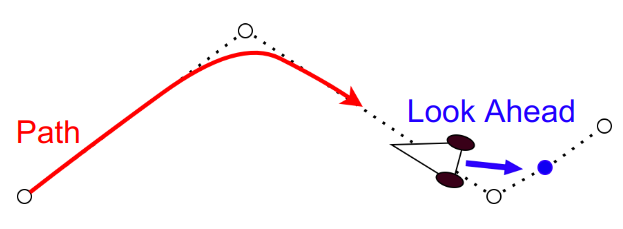
\includegraphics[keepaspectratio, scale=0.5]
      {images/PurePursuit.png}
 \caption{PurePursuit Algorithm}
 \label{fig:purepursuit}
\end{figure}

\subsection{PID制御}
PID制御(Proportional-Integral-Differential Controller)は, 制御工学におけるフィードバック制御の一種である.
出力値と目標値との偏差, その積分, および微分の3つの要素によって, 入力値の制御を行う方法である.

\subsubsection{P制御}
基本的なフィードバック制御として比例制御(P制御)がある.
これは操作量を制御量と目標値の偏差の一次関数として制御するものである.
PID制御では, この偏差に比例して操作量を変化させる動作を比例動作, またはP動作といい, その時の定数は比例ゲイン, Pゲインと呼ばれる.

\subsubsection{I制御}
P制御において, 周囲の環境が変わるたびに残留偏差をなくすように比例ゲインを決定しなおすことが難しい.
そこで, 残留偏差が存在する場合, その偏差の時間積分に比例して入力値を変化させる動作をする項を追加する.
追加した項が持つ役割がI制御である.
偏差のある状態が長い時間続けばそれだけ入力値の変化を大きくして目標値に近づけようとする役目を果たす.
ここで, 定数は積分ゲイン, Iゲインと呼ばれる.

\subsubsection{D制御}
PI制御の問題点として, 周囲の環境が変化したり制御対象に撹乱が加わったりすることで出力値が急に変動することがある.
この問題を解決するために, 急激な出力値の変化が起こった場合, その変化の大きさに比例した入力を行うことでその変化に抵抗する役割を持つ項を追加する.
追加した項が持つ役割がD制御である.
定数は微分ゲイン, Dゲインと呼ばれる.

\section{経路生成}
経路追従を行うためには, 追従するための目標経路(Path)を設定する必要がある.
自律移動ロボットの開発に置いて目標経路の探索を経路計画と呼び, 重要な問題の一つとされている.
本研究では, 目標経路は予め取得した測地座標系の経緯度で用意されたウェイポイントをつなぐライン上で定めている.


\subsection{スプライン補間}
本研究で取得する目標経路は, ウェイポイントを繋ぐライン上で定めている.
定めたウェイポイントが疎らである場合に, ロボットに無理のない追従を行わせるためには目標経路の曲線が滑らかである必要がある.
そこで, 3次スプライン補間を行うことで, 用意されたウェイポイント上を繋ぐラインに対して曲線を担保することが可能となる.

3次スプライン補間とは, 複数のサンプル点が与えられた時に, そのサンプル点の間を3次の多項式で近似し, 滑らかに保管する手法である.
Fig.3.2にその様子を示す.

\begin{figure}[H]
     \centering
    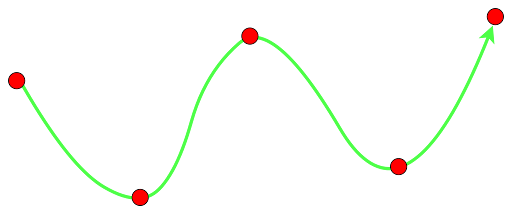
\includegraphics[keepaspectratio, scale=0.5]
         {images/splinepath.png}
    \caption{Spline path}
    \label{fig:purepursuit}
\end{figure}


\newpage
% 4章
\capter{システムの要件}
ここでは, 経路追従を行うシステムに求められる要件を示す.
% 5章
\chapter{実験}
% 6章
\chapter{結論}
